% Figura cuerpo B3 (4.1.5): por qué el objetivo no es cero: el colchón sobre el suelo de los tipos
\documentclass[tikz,border=3pt]{standalone}
\usepackage[T1]{fontenc}
\usepackage[utf8]{inputenc}
\usepackage{amsmath}
\usetikzlibrary{arrows.meta,calc,positioning}
\begin{document}
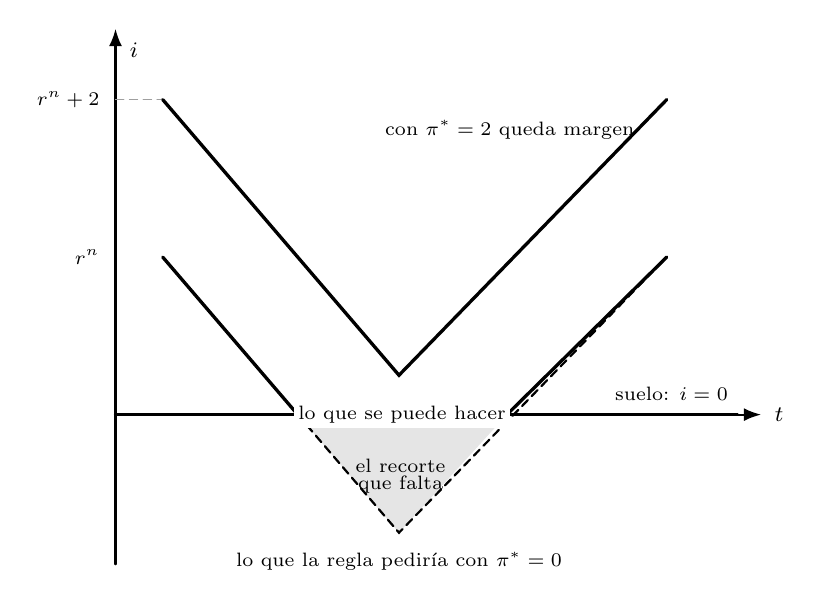
\begin{tikzpicture}[>={Latex[length=2.2mm]}, line cap=round, font=\footnotesize,
  eje/.style={->, thick},
  real/.style={very thick},
  pide/.style={thick, densely dashed},
  guia/.style={densely dashed, gray!75}]

  % Zona imposible
  \fill[black!10] (2.314,0) -- (3.6,-1.5) -- (4.971,0) -- cycle;

  \draw[eje] (0,0) -- (8.2,0);
  \node[anchor=west] at (8.25,0) {$t$};
  \draw[eje] (0,-1.9) -- (0,4.9) node[below right=2pt]{$i$};
  \draw[very thick] (0,0) -- (7.9,0);
  \node[anchor=south east, font=\scriptsize] at (7.9,0.06) {suelo: $i=0$};

  \draw[guia] (0,4.0) -- (0.6,4.0);
  \node[anchor=east, font=\scriptsize] at (-0.08,4.0) {$r^{n}+2$};
  \node[anchor=east, font=\scriptsize] at (-0.08,2.0) {$r^{n}$};

  % Con objetivo del 2 por ciento: queda margen
  \draw[real] (0.6,4.0) -- (3.6,0.5) -- (7.0,4.0);
  \node[anchor=west, font=\scriptsize] at (3.30,3.62) {con $\pi^{*}=2$ queda margen};

  % Con objetivo cero: lo que la regla pediria y lo que se puede hacer
  \draw[pide] (0.6,2.0) -- (3.6,-1.5) -- (7.0,2.0);
  \node[anchor=north, font=\scriptsize, align=center] at (3.6,-1.62) {lo que la regla pediría con $\pi^{*}=0$};
  \draw[real] (0.6,2.0) -- (2.314,0) -- (4.971,0) -- (7.0,2.0);
  \node[fill=white, inner sep=1.6pt, font=\scriptsize] at (3.64,0) {lo que se puede hacer};

  \node[font=\scriptsize, align=center] at (3.62,-0.78) {el recorte\\[-2pt]que falta};

\end{tikzpicture}
\end{document}
